\subsection{Lösungsansatz: Prediktive Kodierung}
Prediktoren sind typische Ansätze für verlustfreie Kompressionsverfahren. Die Frage ist, wie Informationen gelöscht werden. In erster Linie werden zwei Subsampling verfahren getestet, ein einfaches Subsampling und das Adaptive Subsampling. Das Adaptive Subsampling ist gut in unwichtige Informationen zu löschen, ist aber schwieriger zu kodieren. Das 

\subsubsection{Variante: einfaches Subsampling}
Für die erste Variante wird das Subsampling des DCT-Lösungsansatzes verwendet. Es reduziert die Punktmenge auf die Anzahl des Ist-Zustands. Die Feldlinien werden mit einer PCA in ein lokales Koordinatensystem transformiert. Im lokalen System können die Koordinaten mit 16 Bit Genauigkeit dargestellt werden. 16 Bit im Koordinatensystem der Sonne reichen nicht aus und führen zu einem grösseren Fehler als der Ist-Zustand.\\
In dieser Variante wird der Einfluss von vier Prediktoren getestet ($x$ sind die Bekannten Punkte und $y$ die Vorhersage):
\begin{itemize}
\item Konstanter Prediktor: Nimmt an, dass der nächste Wert im Kanal gleich dem  letzten Wert ist ($x = y$).
\item Linearer Prediktor: Nimmt an, dass die Steigung die Steigung zum nächsten Wert konstant bleibt ($x_1+(-x_2+x_1) = y$).
\item Linearer Prediktor mit Moving Average: Nimmt die durchschnittliche Steigung der letzten Werte.
\item Adaptiver Linearer Prediktor mit Moving Average: Berücksichtigt den Fehler der letzten Vorhersage.
\end{itemize}

\begin{figure}[!htbp]
	\center
	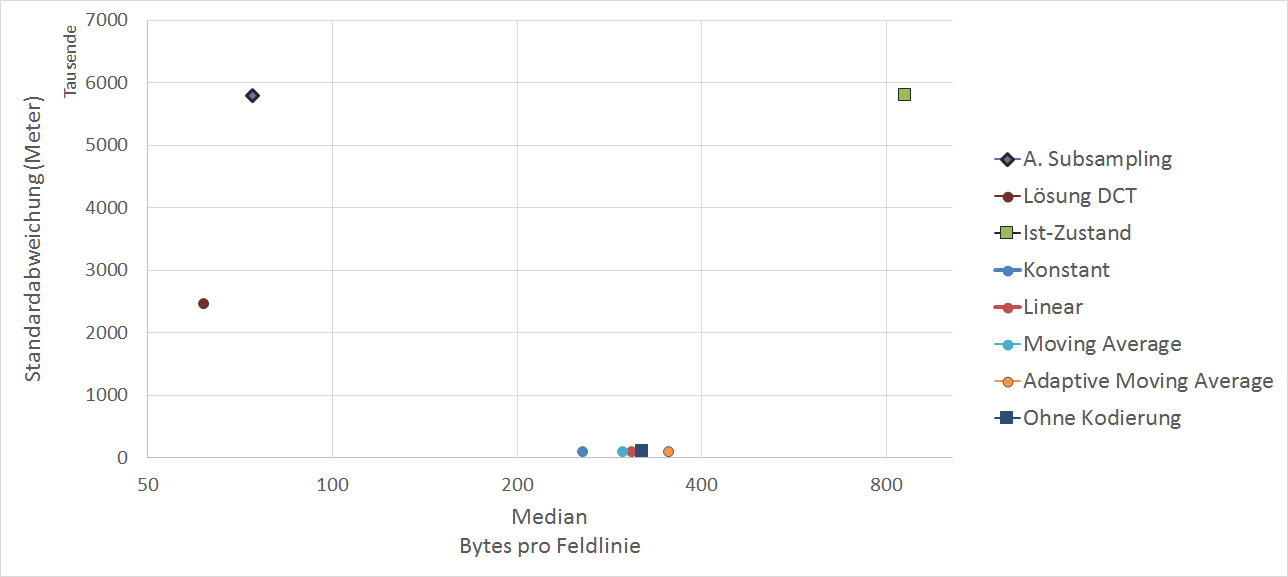
\includegraphics[width=1\textwidth,keepaspectratio]{./pictures/resultate/loesung2/variante0/resultate.png}
	\caption{Kompressionsraten der vier Prediktoren im Vergleich zum Ist-Zustand.}
	\label{resultate:loesung2:simple:resultate}
\end{figure}
Im Diagramm der Abbildung \ref{resultate:loesung2:simple:resultate} sind die Kompressionsraten der jeweiligen Prediktoren dargestellt. Ein Diagramm mit der PSNR-HVS-M wurde nicht erstellt. Sie ist für alle Prediktoren gleich und liegt bei $140.7$ dB. Unerwartet ist, dass der Konstante Prediktor mit $255$ Bytes pro Feldlinie die beste Kompression erreichte, obwohl die Daten nicht zuverlässig vorhersagen kann. Im Vergleich mit dem Moving Average Prediktor sind die Fehler der Vorhersagen 
bis zu $5$ Mal grösser, verbrauchen aber $40$ Bytes weniger um eine Feldlinie abzuspeichern. Der Fehler bleibt jedoch Konstant. Eine Möglichkeit ist, dass die Rar Kodierung sich wiederholende Muster findet.\\
Eine mögliche Optimierung ist die Adaptive Byte Kodierung der DCT-Variante, beschrieben im Abschnitt \ref{konzept:loesung1:kodierung}. Das Diagramm der Abbildung \ref{resultate:loesung2:simple:resultate_byte} zeigt die Resultate mit der Byte Kodierung. Der Konstante Prediktor verbraucht mit der Adaptiven Kodierung mehr Speicherplatz. Die Kompressionsrate der anderen Prediktoren wird durch die Adaptive Kodierung deutlich verbessert. Der Lineare Prediktor erreicht mit $214$ Bytes pro Feldlinie die beste Kompression. Das bedeutet, dass die Fehler des Konstanten Prediktors grösser sind, als die der anderen Prediktoren. Es bestätigt die Vermutung, dass die anderen Prediktoren die Daten besser vorhersagen können. Die Kompressionsrate des Konstanten Prediktors ist auf die Rar Kodierung zurückzuführen, welche in den Prediktor-Fehler Muster erkennen und effizient kodieren kann.\\ 
\begin{figure}[!htbp]
	\center
	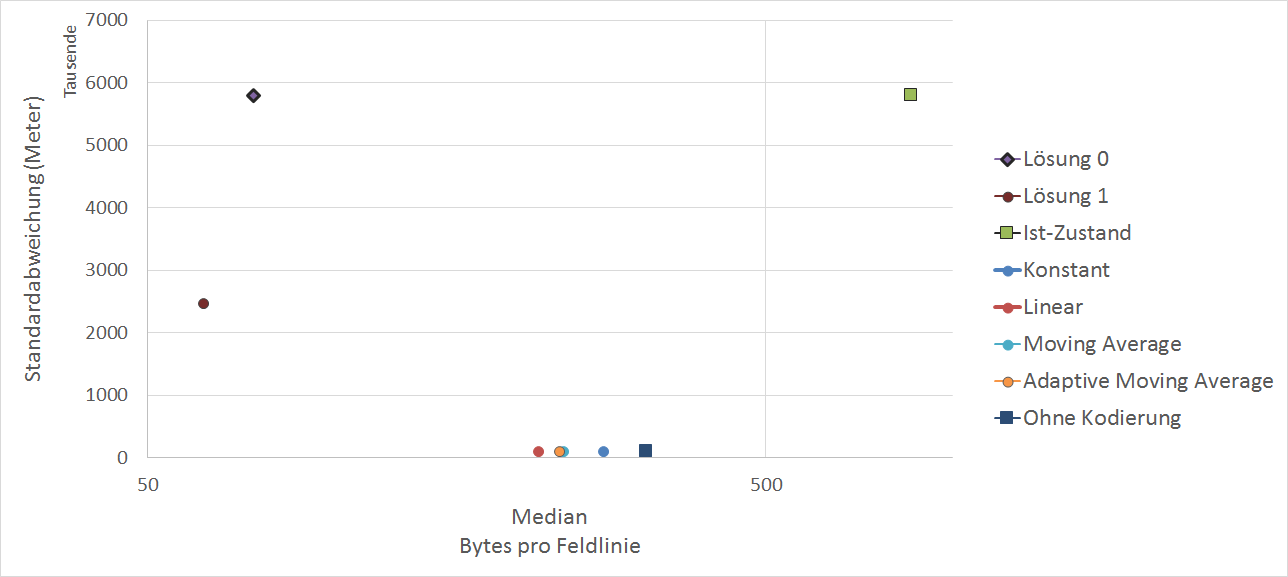
\includegraphics[width=1\textwidth,keepaspectratio]{./pictures/resultate/loesung2/variante0/resultate_byte.png}
	\caption{Kompressionsraten der Prediktoren mit Adaptiver Byte Kodierung.}
	\label{resultate:loesung2:simple:resultate_byte}
\end{figure}
Der Linare Prediktor kann eine Feldinie mit etwa $214$ Bytes darstellen, was eine Kompressionsrate von $4$ ergibt.

\subsubsection{Variante: Adaptives Subsampling}
Um mit diesem Ansatz in die selbe Grössenordnung zu gelangen wie die Lösungsansätze Adaptives Subsampling und DCT müssen mehr Informationen gelöscht werden. Es werden andere Parameter verwendet und im Schnitt $50\%$ mehr Punkte übertragen als im Lösungsansatz des Adaptiven Subsampling.\\
\begin{figure}[!htbp]
	\center
	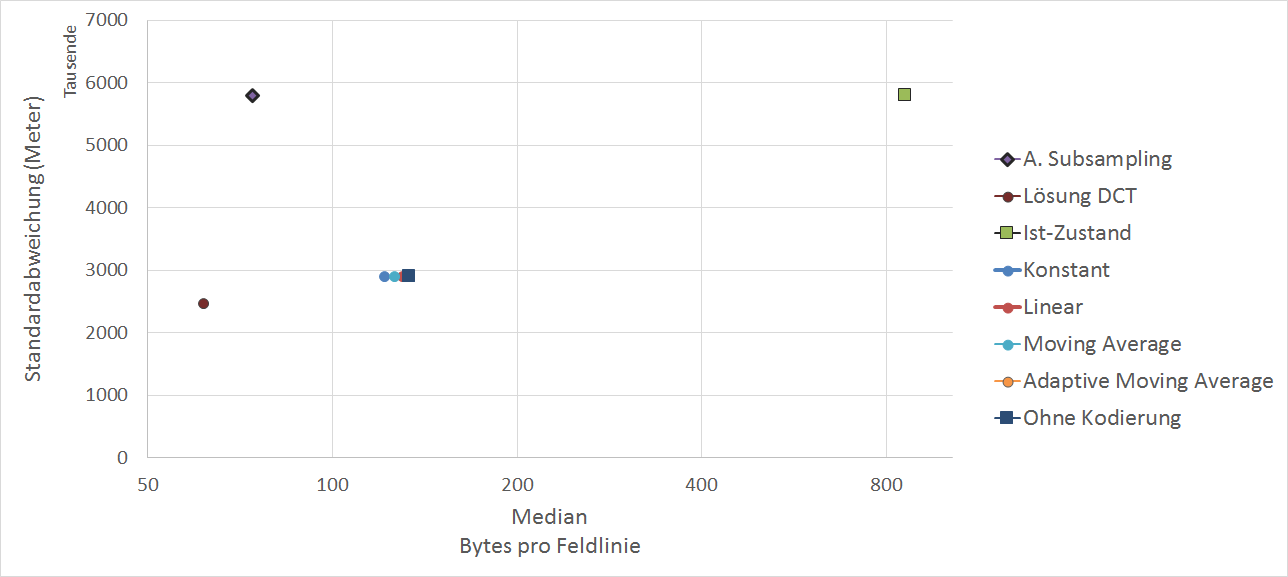
\includegraphics[width=1\textwidth,keepaspectratio]{./pictures/resultate/loesung2/variante1/resultate_euler.png}
	\caption{Kompressionsraten der Prediktiven Kodierungen mit dem adaptiven Subsampling.}
	\label{resultate:loesung2:adaptive:euler}
\end{figure}
Das Diagramm der Abbildung \ref{resultate:loesung2:adaptive:euler} zeigt die Kompressionsraten. Die Resultate liegen dicht beieinander und der Abstand zwischen Kodierung und der Kompression, welche ohne Kodierung erreicht wird wurde drastisch vermindert. Die Kodierungen erreichen eine PSNR-HVS-M von $139,2$. Das Angle Subsampling verändert die Eigenschaften der Daten. Die Diagramme der Abbildung \ref{resultate:loesung2:adaptive:channel} visualisiert die Veränderung. Monotone Steigungen sind nach dem Subsampling nicht mehr vorhanden. Die einfachen Prediktoren können die Daten nicht zuverlässig vorhersagen. 
\begin{figure}[!htbp]
	\center
	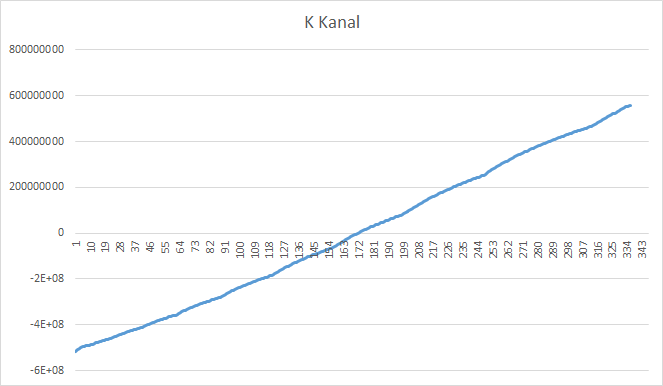
\includegraphics[width=0.49\textwidth,height=5cm,keepaspectratio]{./pictures/resultate/loesung2/variante1/channel_sub.png}
	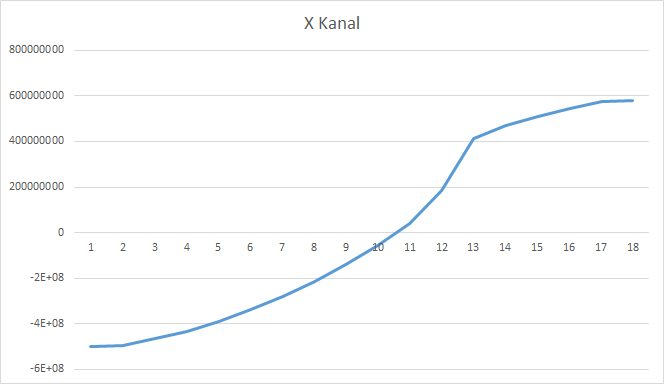
\includegraphics[width=0.49\textwidth,height=5cm,keepaspectratio]{./pictures/resultate/loesung2/variante1/channel_angle.png}
	\caption{Änderung der Eigenschaften der Daten durch das Angle Subsampling. Links der Kanal einer Feldlinie vor, rechts der Kanal nach dem Angle Subsampling.}
	\label{resultate:loesung2:adaptive:channel}
\end{figure}

\subsubsection{Rekursive Lineare Kodierung}
Die Rekursive Lineare Kodierung ist in der Lage nicht-stetigen Kanälen eine sinnvolle Vorhersage zu berechnen. Das Verfahren ist im Abschnitt \ref{konzept:prediktiv} genauer erleutert. Die Punkte werden ins sphärische Koordinatensystem überführt. In diesem Koordinatensystem sind 16 Bit Genauigkeit pro Koordinatenachse ausreichend und die PCA muss nicht berechnet werden. Im Schnitt können dadurch $30$ Bytes pro Feldlinie eingespart werden. 
Zusätzlich werden die Vorhersagefehler quantisiert. Bei den einfachen Prediktoren wurde keine Quantisierung des Fehlers vorgenommen. Jede Quantisierung führte zu einem markanten Anstieg der Abweichung.\\
\begin{figure}[!htbp]
	\center
	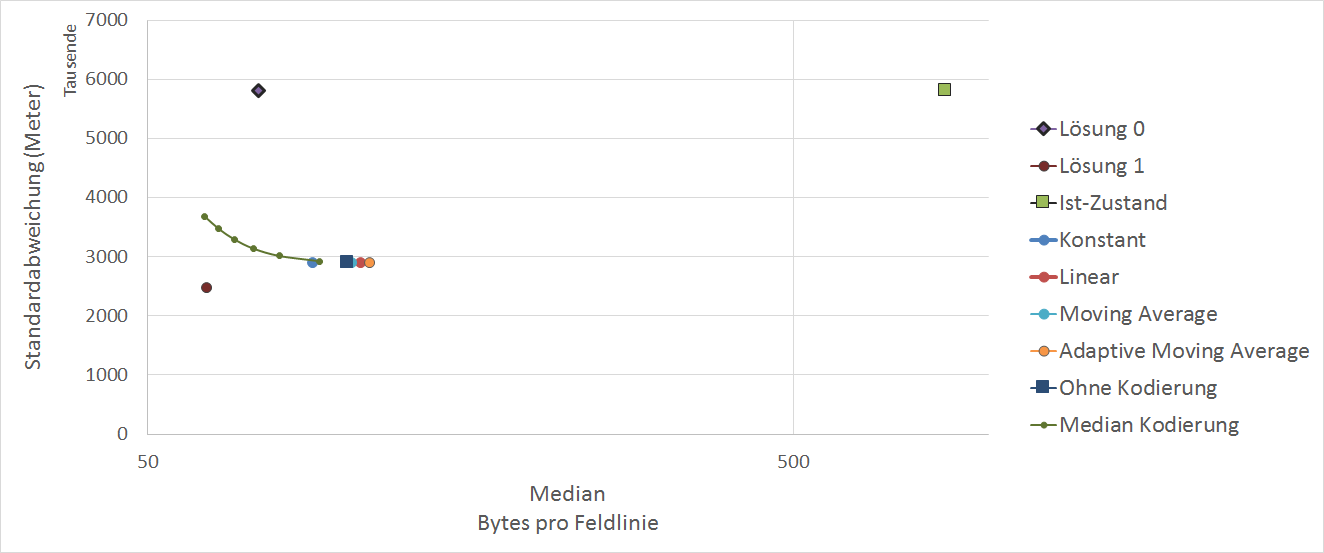
\includegraphics[width=1\textwidth,keepaspectratio]{./pictures/resultate/loesung2/variante2/resultate.png}
	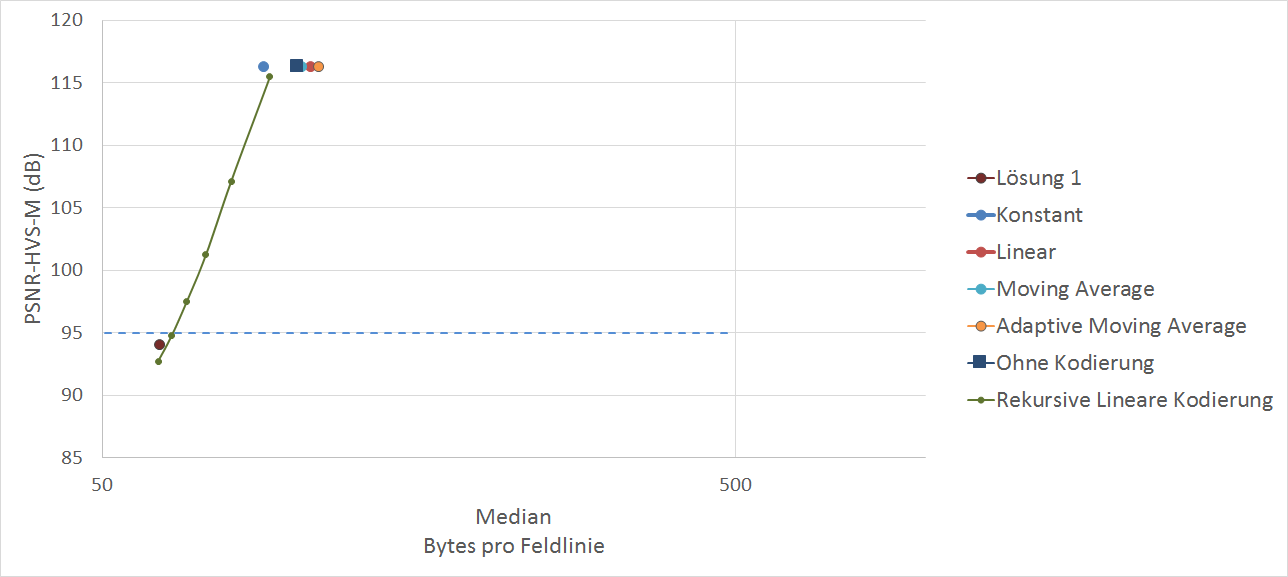
\includegraphics[width=1\textwidth,keepaspectratio]{./pictures/resultate/loesung2/variante2/resultate_psnr.png}
	\caption{Kompressionsraten der Rekursive Lineare Kodierung mit dem adaptiven Subsampling.}
	\label{resultate:loesung2:adaptive:median}
\end{figure}
Das Diagramm der Abbildung \ref{resultate:loesung2:adaptive:median} zeigt die Standardabweichung und PSNR-HVS-M der Rekursiven Linearen Kodierung zu unterschiedlichen Quantisierungen. Die Resultate der einfachen Prediktoren wurden ebenfalls ohne PCA im sphärischen Koordinatensystem gemessen. Die Rekursive Lineare Kodierung kann eine bessere Kompressionsrate erreichen als die Lösung des Adaptiven Subsamplings. Bei Datenmenge von $68$ Bytes pro Feldlinie erreicht diese Variante eine tiefere Standardabweichung als das Adaptive Subsampling und eine höhere PSNR-HVS-M als die DCT Lösung. Die DCT Lösung weist eine tiefere Standardabweichung auf. Die Variante ereicht eine Kompressionsrate von $12.6$ und fällt somit zwischen den Lösungsansätzen DCT und Adaptives Subsampling.

Die Artefakte der Dekompression äussern sich meist als leichte Verschiebungen einzelner Punkte. Ein Extremfall führte zu Ringing ähnlichen Artefakte, welche in der Abbildung \ref{resultate:loesung2:adaptive:median:artefakte} dargestellt sind. Die Artefakte entstehen durch das Runden der quantisierten Vorhersagefehler. Die Artefakte aus Abbildung \ref{resultate:loesung2:adaptive:median:artefakte} entstehen, wenn die Nachkommastellen abgeschnitten werden. Die Artefakte, welche durch das Abschneiden entstehen, am schwierigsten vom blossen Auge zu erkennen. Durch eine Glättung können die Artefakte beinahe komplett versteckt werden.
\begin{figure}[!htbp]
	\center
	\frame{
	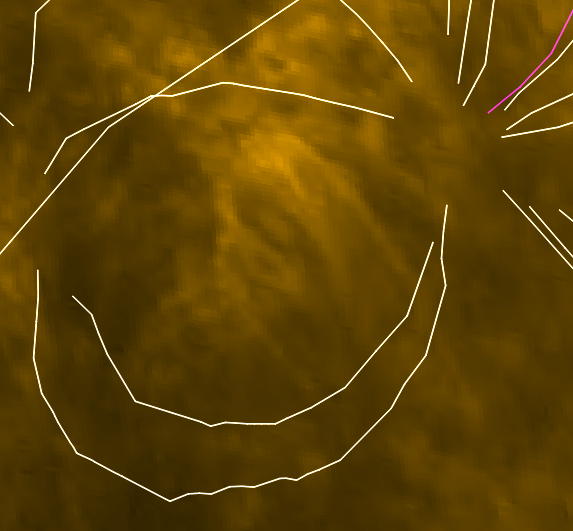
\includegraphics[width=0.8\textwidth,height=5cm,keepaspectratio]{./pictures/resultate/loesung2/variante2/artefakte1.png}}
		\frame{
	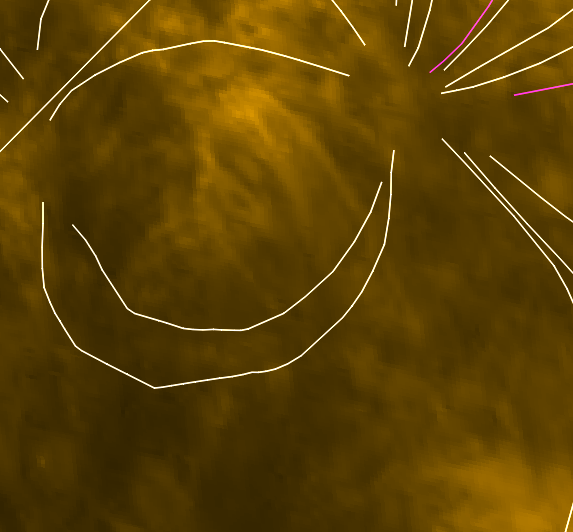
\includegraphics[width=0.8\textwidth,height=5cm,keepaspectratio]{./pictures/resultate/loesung2/variante2/artefakte2.png}}
	\caption{Artefakte der Rekursiven Linearen Kodierung. Links ohne Glättung, rechts mit Glättung}
	\label{resultate:loesung2:adaptive:median:artefakte}
\end{figure}
